\documentclass{beamer}
\usepackage[utf8]{inputenc}
\usepackage{beamerthemesplit}
\usepackage{graphicx}
\usepackage{mathtools}

\usetheme{Madrid}
\usecolortheme{whale}
\beamertemplatenavigationsymbolsempty

\DeclareMathOperator*{\argmax}{arg\,max}
\DeclareMathOperator*{\argmin}{arg\,min}

\title{\textbf{Dense range images from sparse point clouds using multi-scale processing}}
\subtitle{Luat Do, Lingni Ma, Peter H.N. de With \quad 2012}
\author{Tim Lenertz / Renzhi Deng}
\date{10 december 2014}
\institute{Université Libre de Bruxelles}

\maketitle

\begin{document}

\begin{frame}
\frametitle{Point cloud projection}
	\begin{columns}
	\begin{column}[T]{.5\textwidth}
		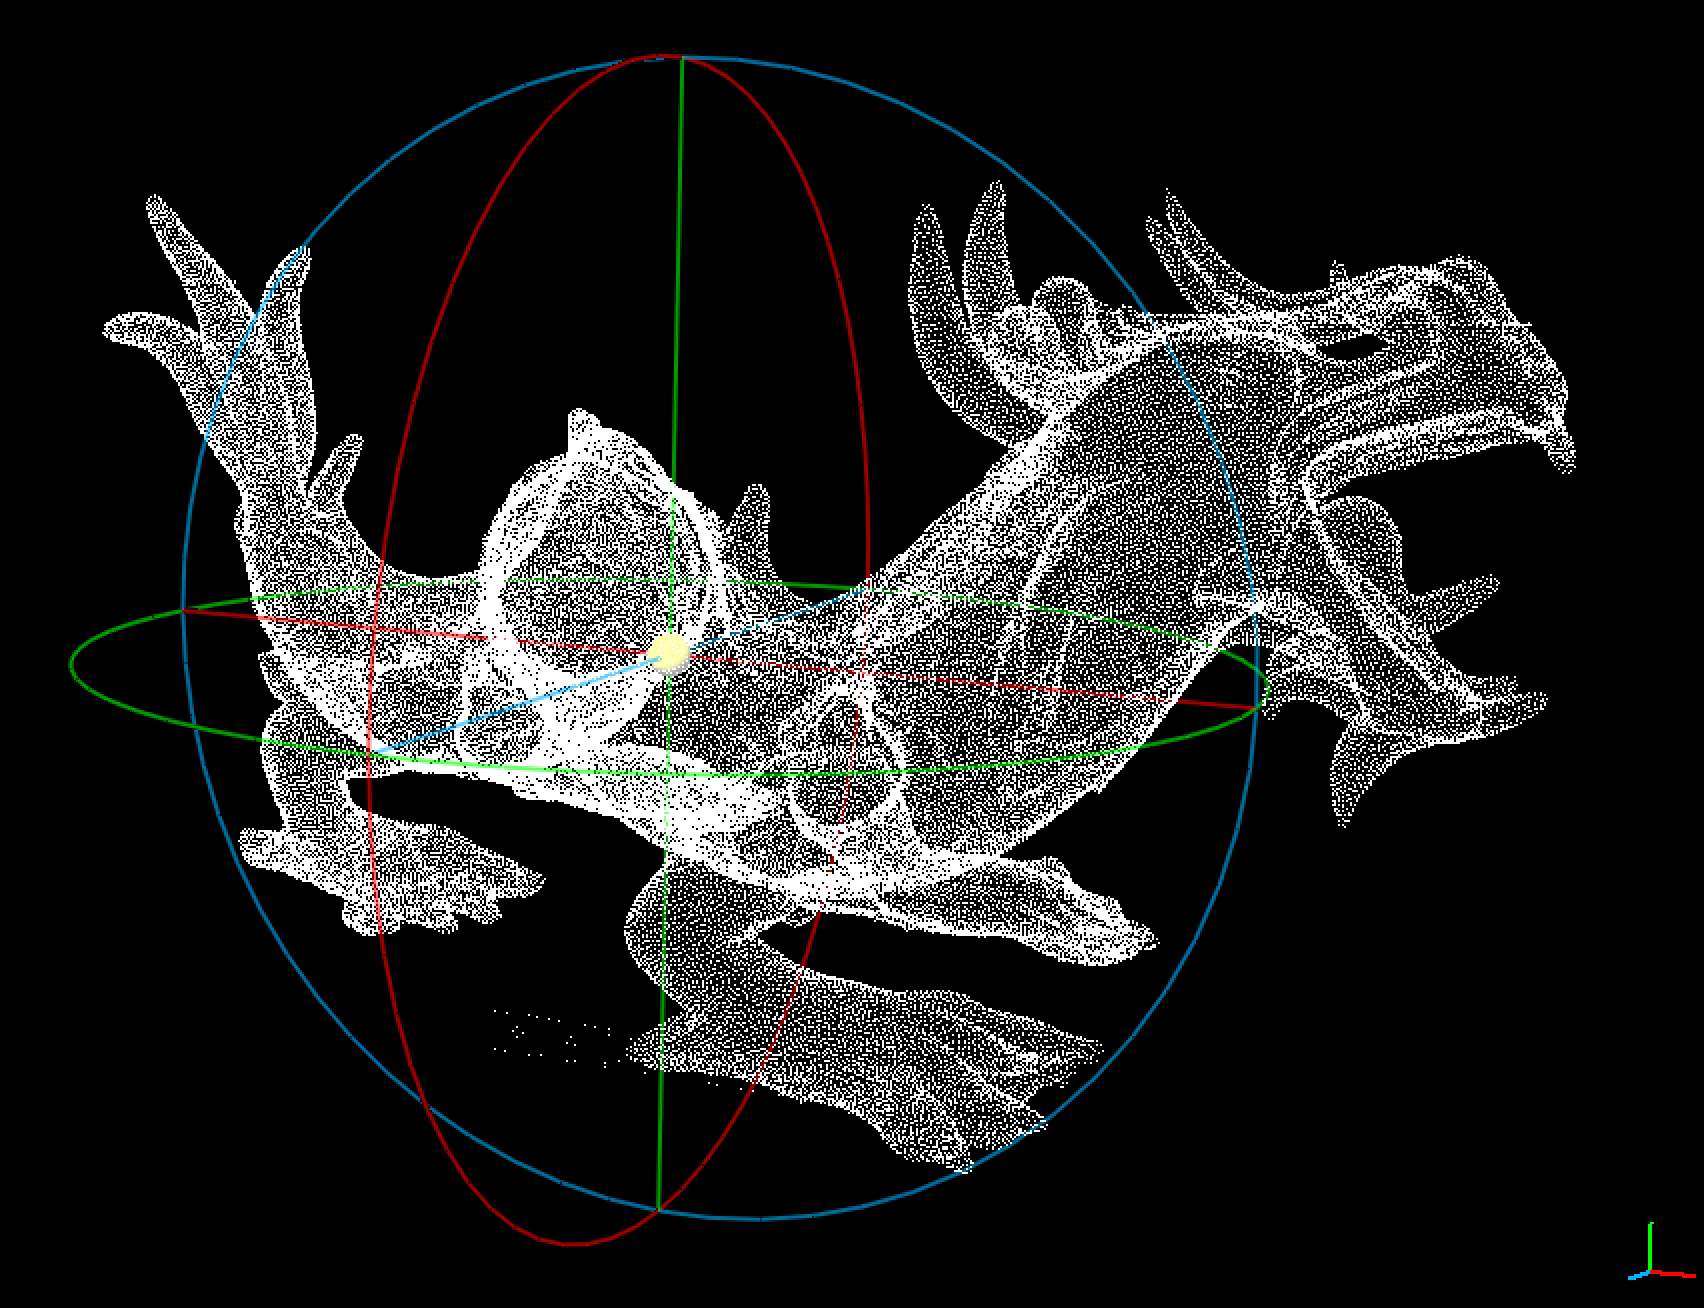
\includegraphics[height=4.3cm]{pointcloud.png}
		\\ \textbf{Point cloud} \\
		Set of X,Y,Z points \\
	\end{column}
	\begin{column}[T]{.5\textwidth}
		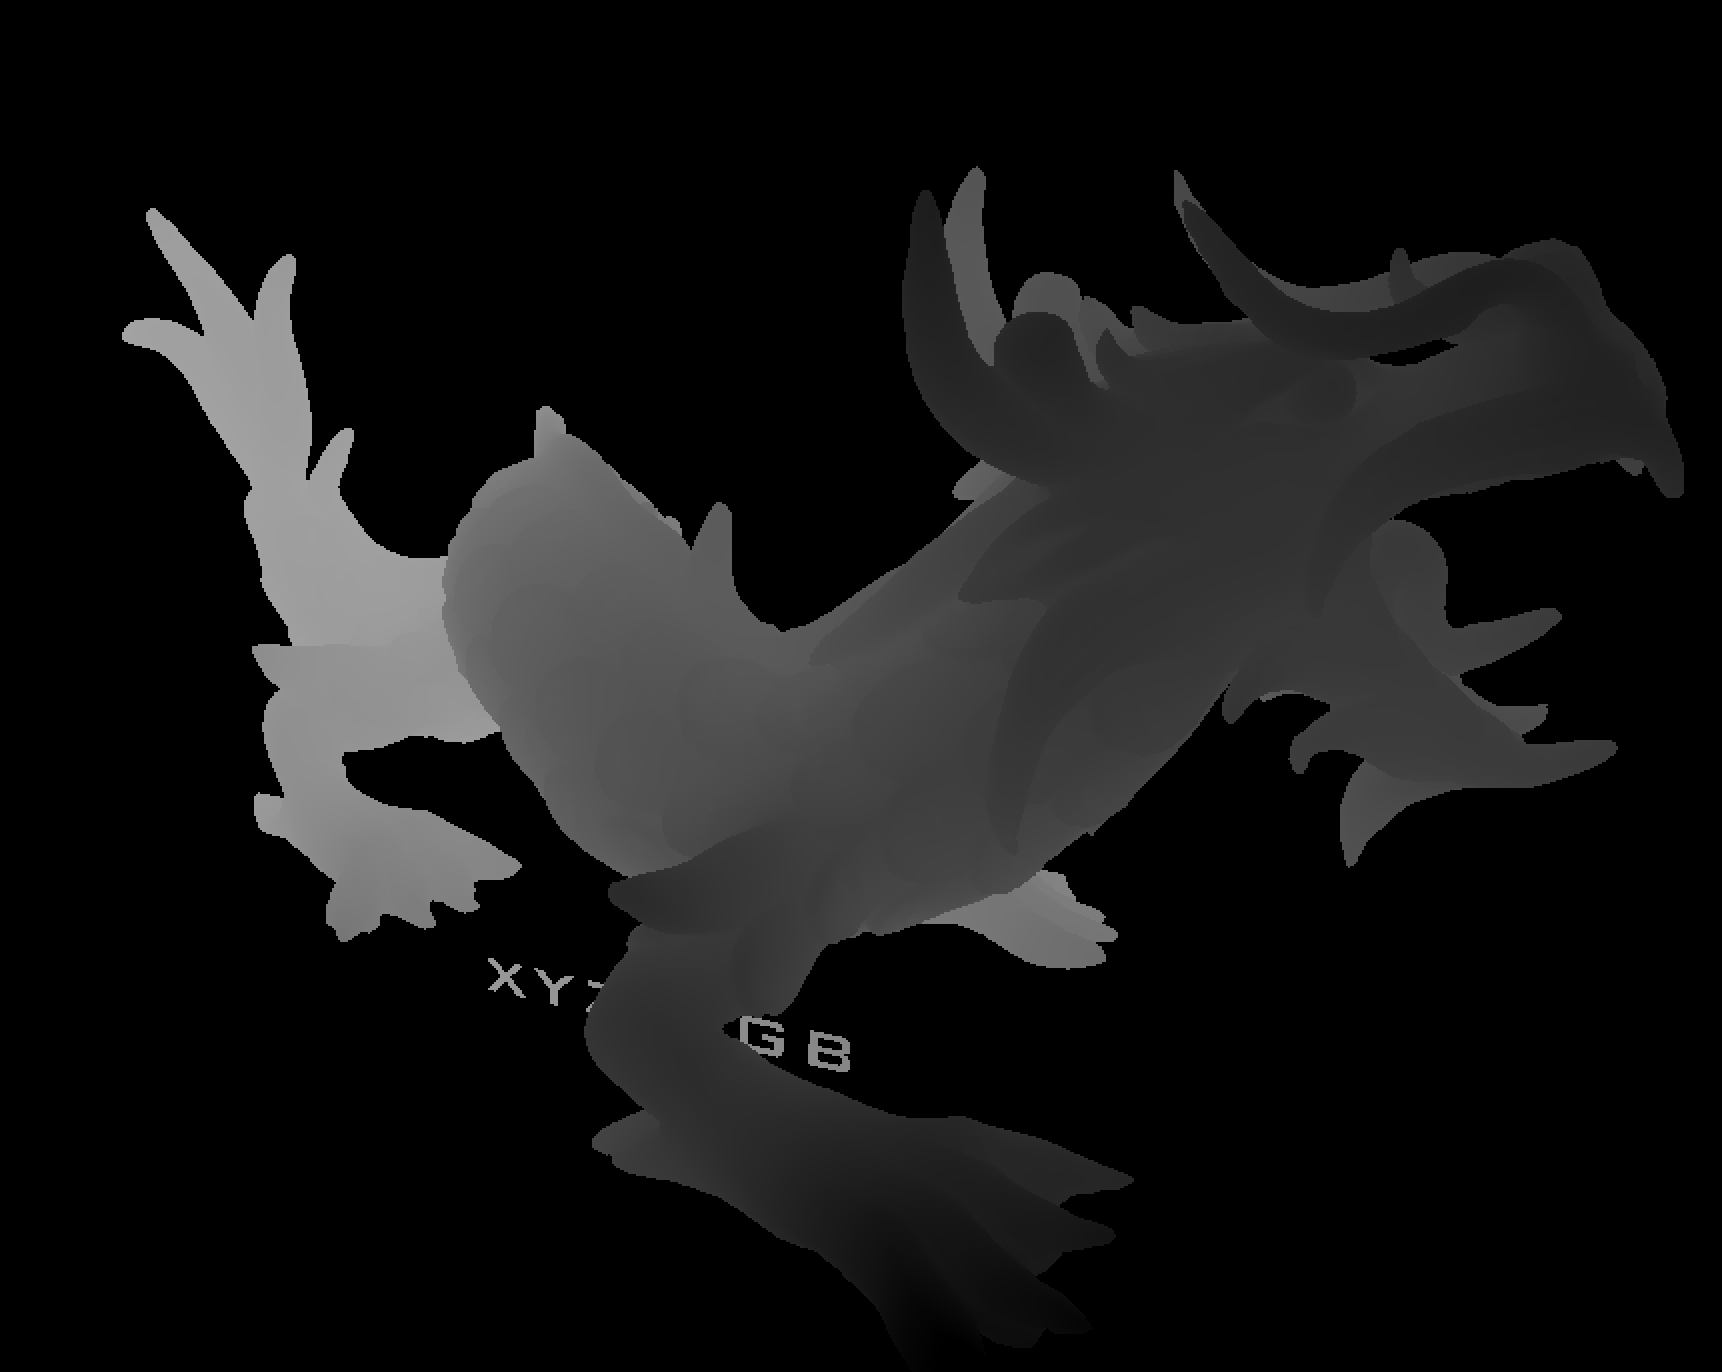
\includegraphics[height=4.3cm]{depthmap.png}
		\\ \textbf{Range image} \\
		Depth values on X,Y grid \\
		Output of 3D scanner \\ \\
		Only information seen from one view point \\
		 \\
	\end{column}
	\end{columns}
\end{frame}


\begin{frame}
\frametitle{Sparse Range Image}
	\begin{columns}
	\begin{column}[T]{.5\textwidth}
		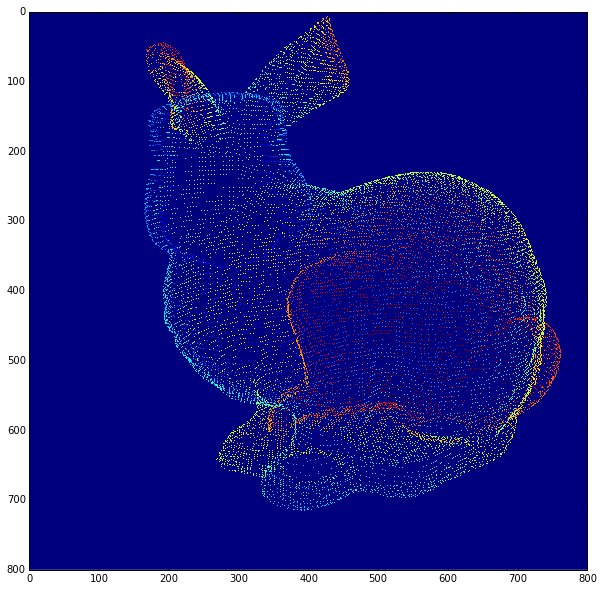
\includegraphics[height=5cm]{high.png}
		\\ \textbf{800x800 pixel} \\
		Sparse \\
		Pixels with no corresp. point
	\end{column}
	\begin{column}[T]{.5\textwidth}
		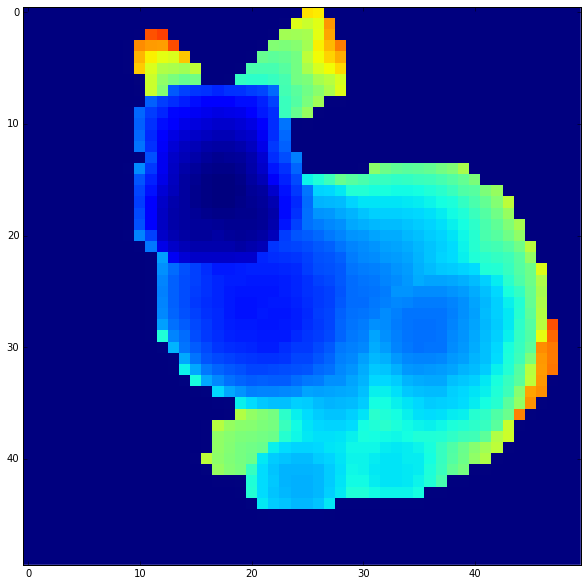
\includegraphics[height=5cm]{low.png}
		\\ \textbf{50x50 pixel} \\
		Dense, no holes \\
		But lower quality \\
	\end{column}
	\end{columns}
	\vspace{.5cm}
	$\rightarrow$ \textbf{Aim:} Combine information from both 
\end{frame}


\frame[plain]{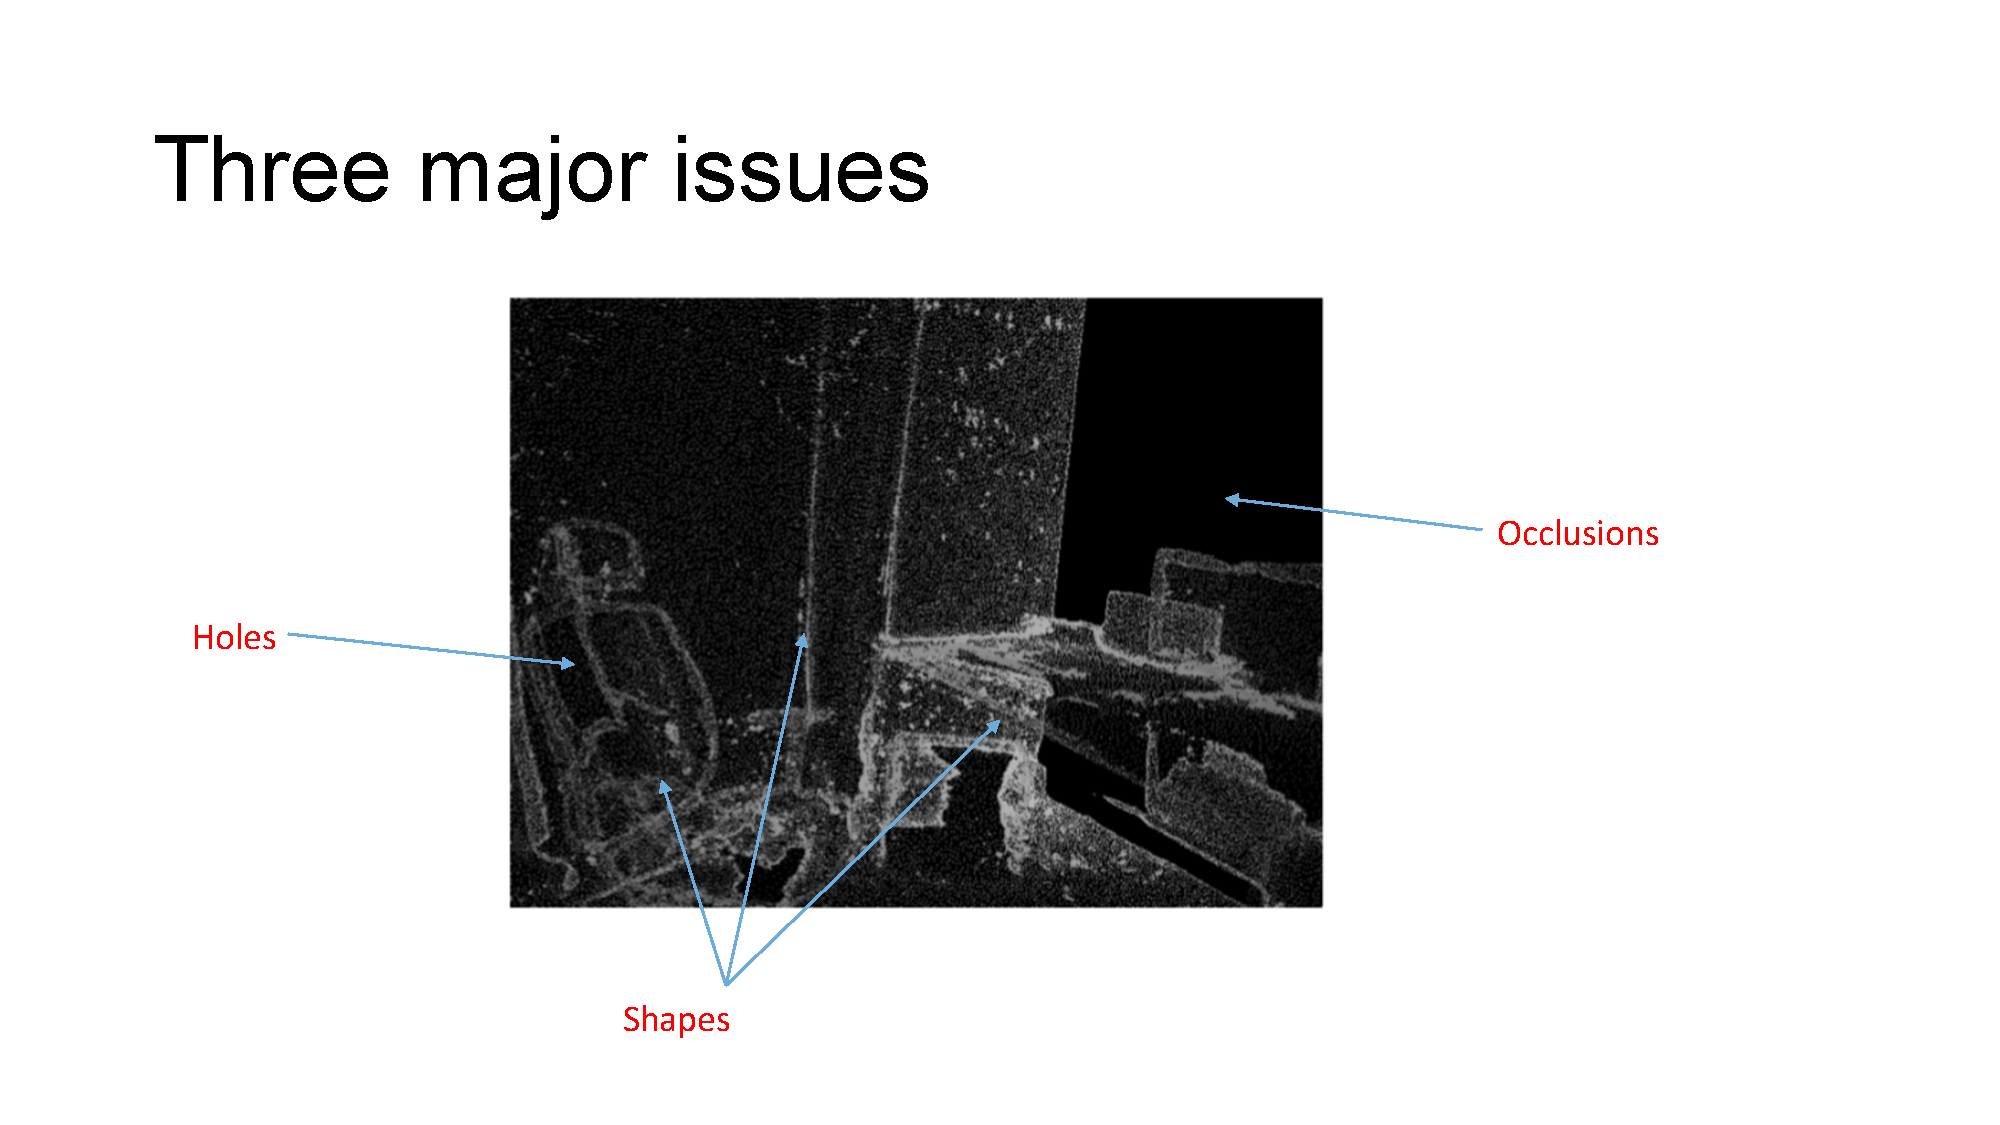
\includegraphics[page=1,width=\textwidth]{superresolution.pdf}}
\frame[plain]{\includegraphics[page=2,width=\textwidth]{superresolution.pdf}}
\frame[plain]{\includegraphics[page=3,width=\textwidth]{superresolution.pdf}}


\begin{frame}
\frametitle{iPython Implementation}
	Results obtained:
	\begin{columns}
	\begin{column}[T]{.5\textwidth}
		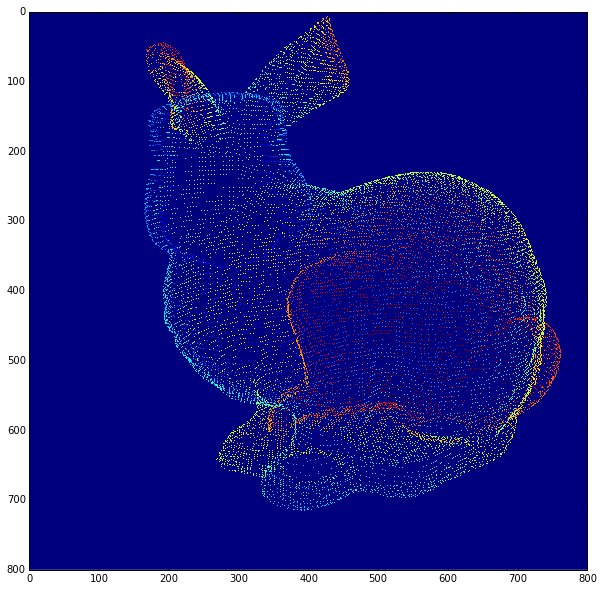
\includegraphics[height=5cm]{res1.png}
		\\ Original sparse projection
	\end{column}
	\begin{column}[T]{.5\textwidth}
		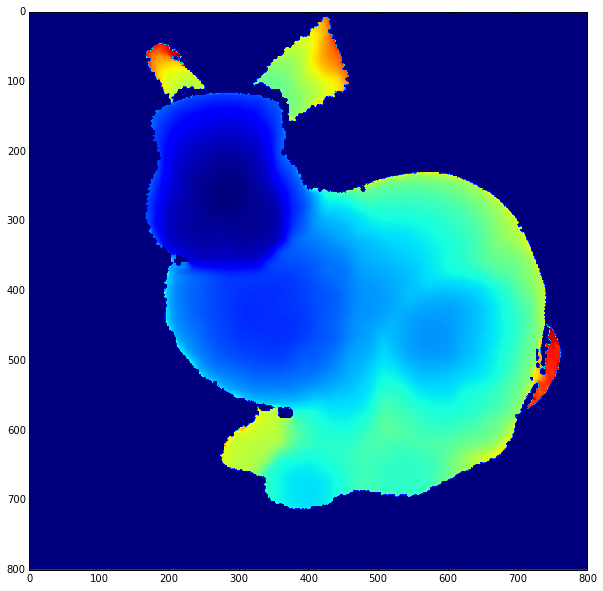
\includegraphics[height=5cm]{res1d.png}
		\\ Result of superresolution algorithm
	\end{column}
	\end{columns}
\end{frame}


\begin{frame}
\frametitle{iPython Implementation}
	Results obtained:
	\begin{columns}
	\begin{column}[T]{.5\textwidth}
		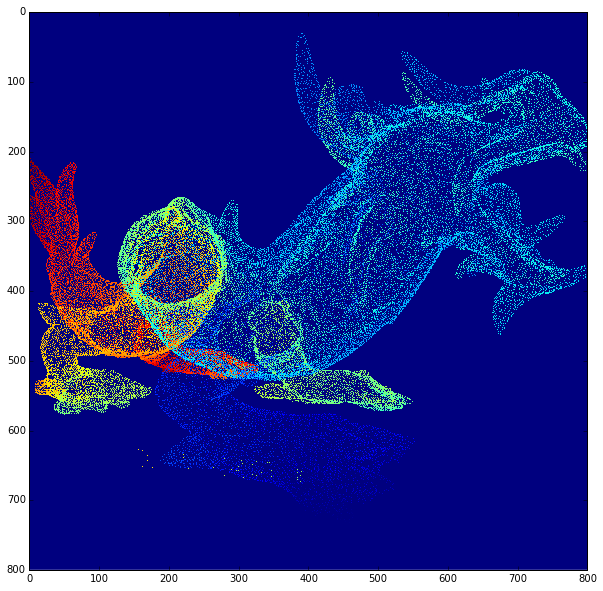
\includegraphics[height=5cm]{res2.png}
		\\ Original sparse projection
	\end{column}
	\begin{column}[T]{.5\textwidth}
		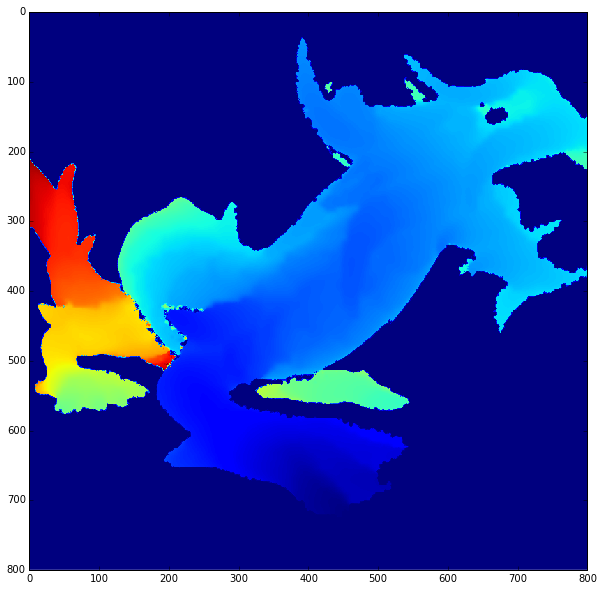
\includegraphics[height=5cm]{res2d.png}
		\\ Result of superresolution algorithm
	\end{column}
	\end{columns}
\end{frame}


\begin{frame}
\frametitle{iPython Implementation}
	\huge{Demo}
\end{frame}


\begin{frame}
\frametitle{Application: Range-Color Image Alignment}
	\begin{columns}
	\begin{column}[T]{.5\textwidth}
		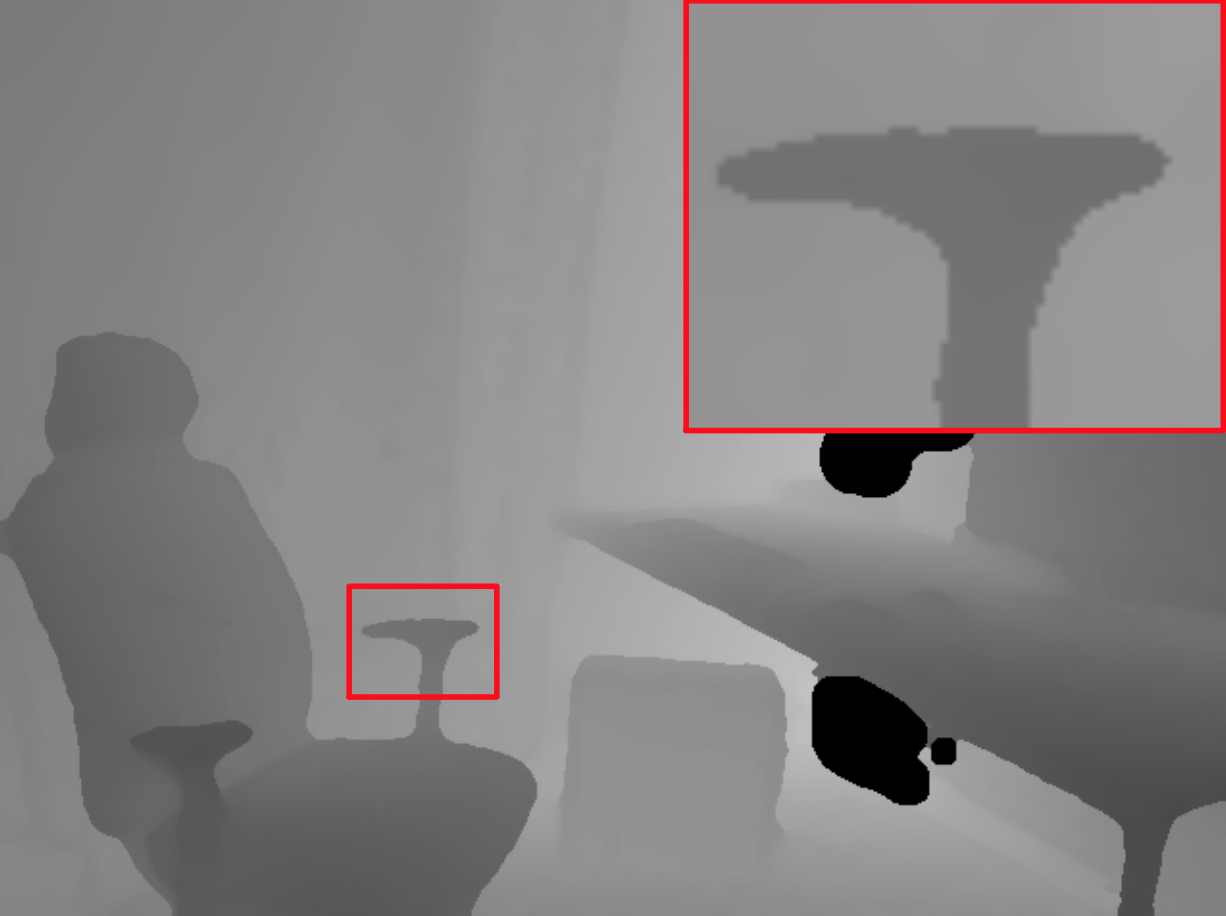
\includegraphics[height=4.5cm]{deskri.png}
		\\ \textbf{Dense range image}
		\\ Output of algorithm
	\end{column}
	\begin{column}[T]{.5\textwidth}
		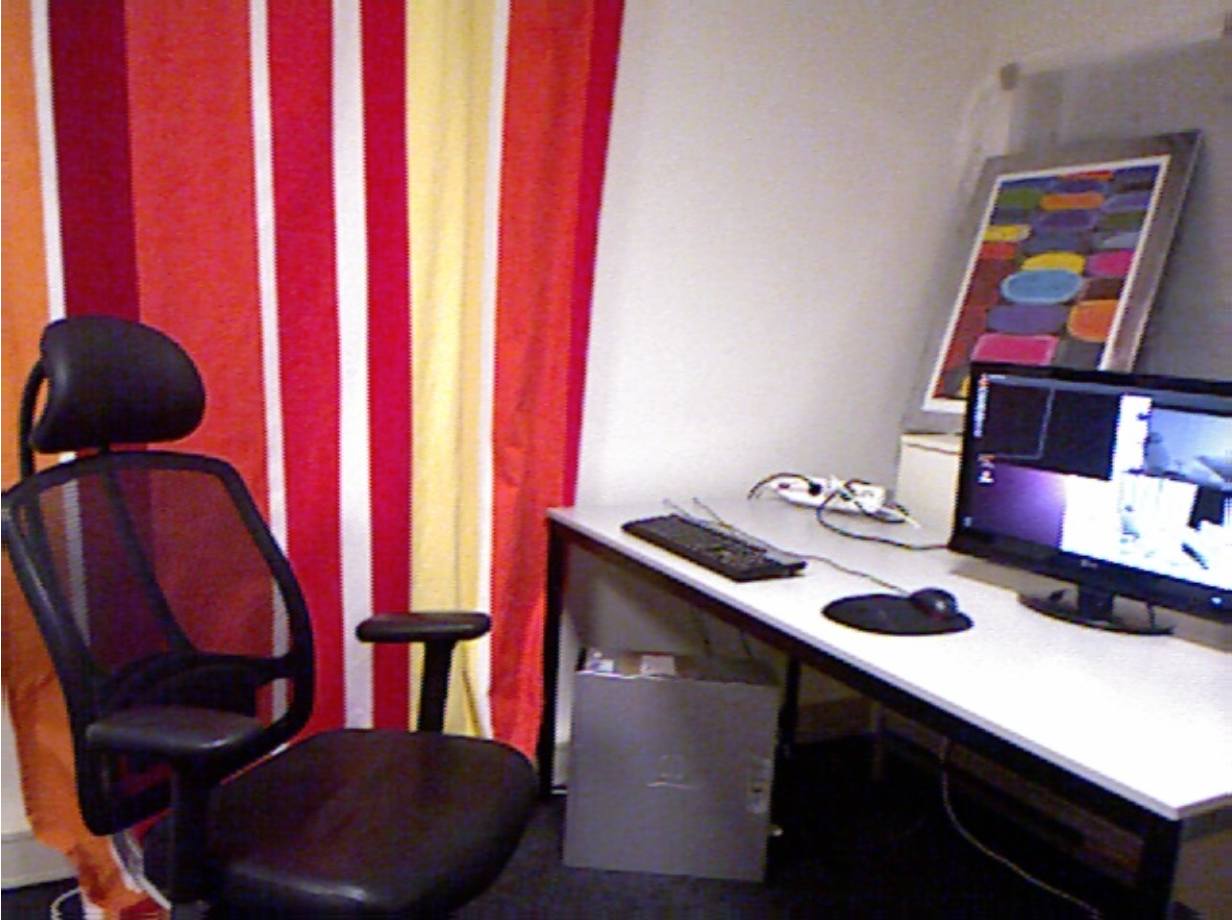
\includegraphics[height=4.5cm]{deskph.png}
		\\ \textbf{Color photograph}
		\\ Slightly different view angle
	\end{column}
	\end{columns}
\end{frame}


\begin{frame}
\frametitle{Application: Range-Color Image Alignment}
	\begin{columns}
	\begin{column}[T]{.7\textwidth}
		\begin{itemize}
		\item Detect edges in both photo and range image
		\item Correspondences of photo \& range edge pixels \\
			$\rightarrow$ Initially: closest on other image
		\item Have 2D-3D pairs (upon backprojection)
		\item Solve Perspective-to-Point equation \\
			\begin{equation*}
			\argmin_{\mathbf{M}} \sum_{i} (\mathbf{P} \mathbf{M} \vec{r_i} - \vec{c_i})^{2}
			\end{equation*}
			$\rightarrow$ find better camera pose $\mathbf{M}$
		\item Project using new $\mathbf{M}$
		\item Apply superresolution, fill holes
		\item Repeat until $\mathbf{M}$ converges
		\end{itemize}
	\end{column}
	\begin{column}[T]{.3\textwidth}
		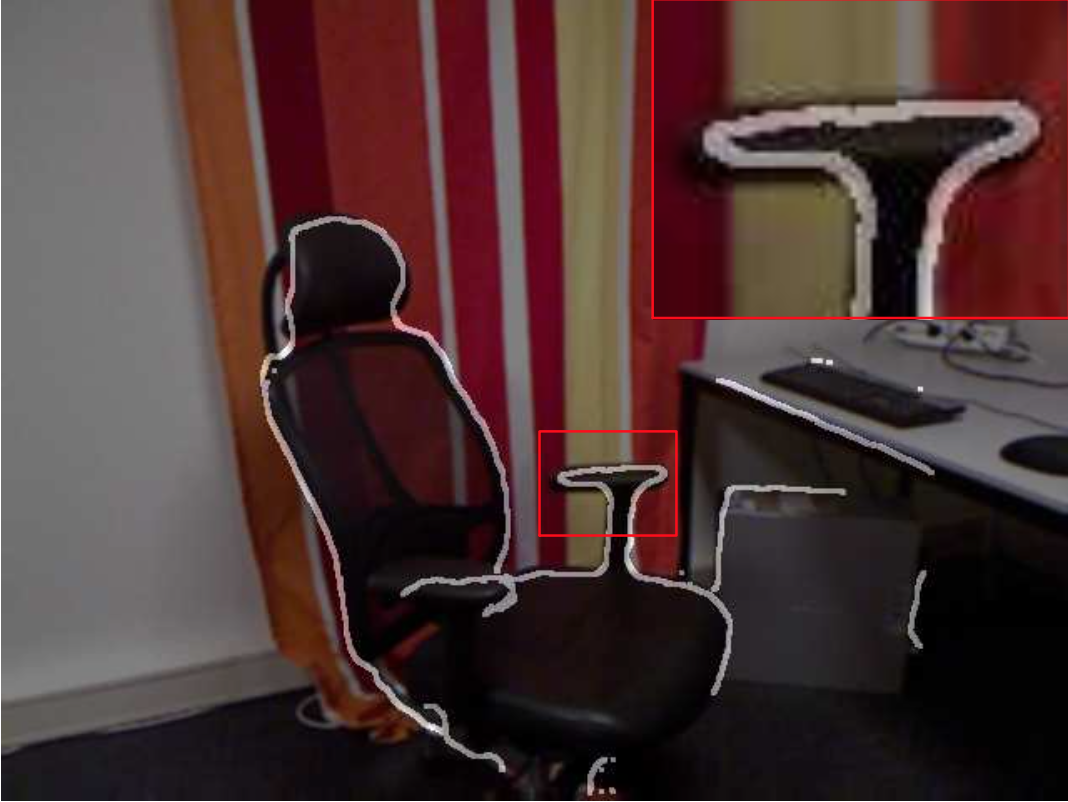
\includegraphics[width=\textwidth]{riedges.png}
	\end{column}
	\end{columns}
\end{frame}

\end{document}
